\chapter{Experimenteel Onderzoek}
\label{ch:experiment}

In het voorgaande hoofdstuk werd de ontwikkeling van de proof-of-concept softwareapplicatie uitvoerig besproken.
Voor ontwikkelingsdoeleinden werd gebruik gemaakt van een dataset die thuis werd opgenomen met de Tobii Pro Glasses 3.
Echter was deze dataset niet geschikt voor evaluatie van de uiteindelijke analysemethoden, aangezien ze door de onderzoeker zelf werden opgenomen en geen objecten bevatten die relevant zijn voor de zorgcontext.
Om een dataset te verkrijgen die wel aan deze kwaliteitseisen voldoet, werd er een experiment opgezet in het Zorglab van HoGent waarin studenten gevraagd om de eyetracker te dragen en te kijken naar verschillende objecten.
De opzet, uitvoering en de resulterende data van dit experiment worden in dit hoofdstuk nader toegelicht.

\section{Doelstellingen van het Experiment}

Het hoofddoel van het experiment was om een dataset te creëren die als grondwaarheid kon dienen voor het valideren van de twee kernmetrieken van de PoC applicatie:
\begin{itemize}
    \item De objecten die de studenten hebben bekeken.
    \item De tijdsduur dat de studenten naar deze objecten hebben gekeken.
\end{itemize}
Om deze validatie mogelijk te maken, werden twee soorten opnames gegenereerd. 
Ten eerste werden er zogenaamde \textit{kalibratieopnames} gemaakt door de onderzoeker zelf. 
Deze dienden primair om de computervisiemodellen binnen de analyses te initialiseren met de visuele kenmerken van de te detecteren objecten. 
Ten tweede werden er \textit{evaluatieopnames} verzameld waarbij studenten de eyetracker droegen en de observatietaak uitvoerden. 
Deze laatste categorie vormt de kern van de te analyseren data waarvoor de ground-truth werd vastgesteld.

Naast het genereren van deze ground-truth, had het experiment ook als doel om de robuustheid van de ontwikkelde analysemethoden te onderzoeken. 
Dit omvatte het evalueren van de prestaties van het systeem onder invloed van verschillende factoren, waaronder:
\begin{itemize}
    \item De invloed van \textbf{variërende kijkafstanden tot objecten} op de detectieaccuraatheid, resulterend in variaties in objectgrootte en detail in het camerabeeld.
    \item De prestaties van de modellen bij \textbf{diverse objectkarakteristieken}, zoals verschillen in vorm, grootte, textuur en mate van transparantie.
    \item De impact van \textbf{wisselende achtergronden} op de betrouwbaarheid van de objectherkenning.
\end{itemize}

\section{Opzet van het Experiment}

De concrete uitwerking van het experiment omvatte de selectie van deelnemers, de inrichting van de experimentele omgeving, de keuze van kritische objecten en een gestandaardiseerde procedure.

\subsection{Experimentele Omgeving en Materialen}

De experimentele opnames vonden plaats in het Zorglab van HOGENT, dat beschikt over verschillende gesimuleerde zorgomgevingen. 
Voor dit onderzoek werd specifiek gebruik gemaakt van de ruimte die is ingericht als een \textbf{woonkameromgeving}. 
Deze setting omvat typische elementen zoals een zithoek met een zetel, een keukengedeelte en een eettafel. 
Hoewel het Zorglab ook een gesimuleerde ziekenhuiskamer met twee bedden ter beschikking stelt, werd omwille van praktische overwegingen, 
zoals de positionering van objecten en de bewegingsvrijheid voor de deelnemers, gekozen voor de woonkameropstelling.

\begin{figure}[H]
  \centering
  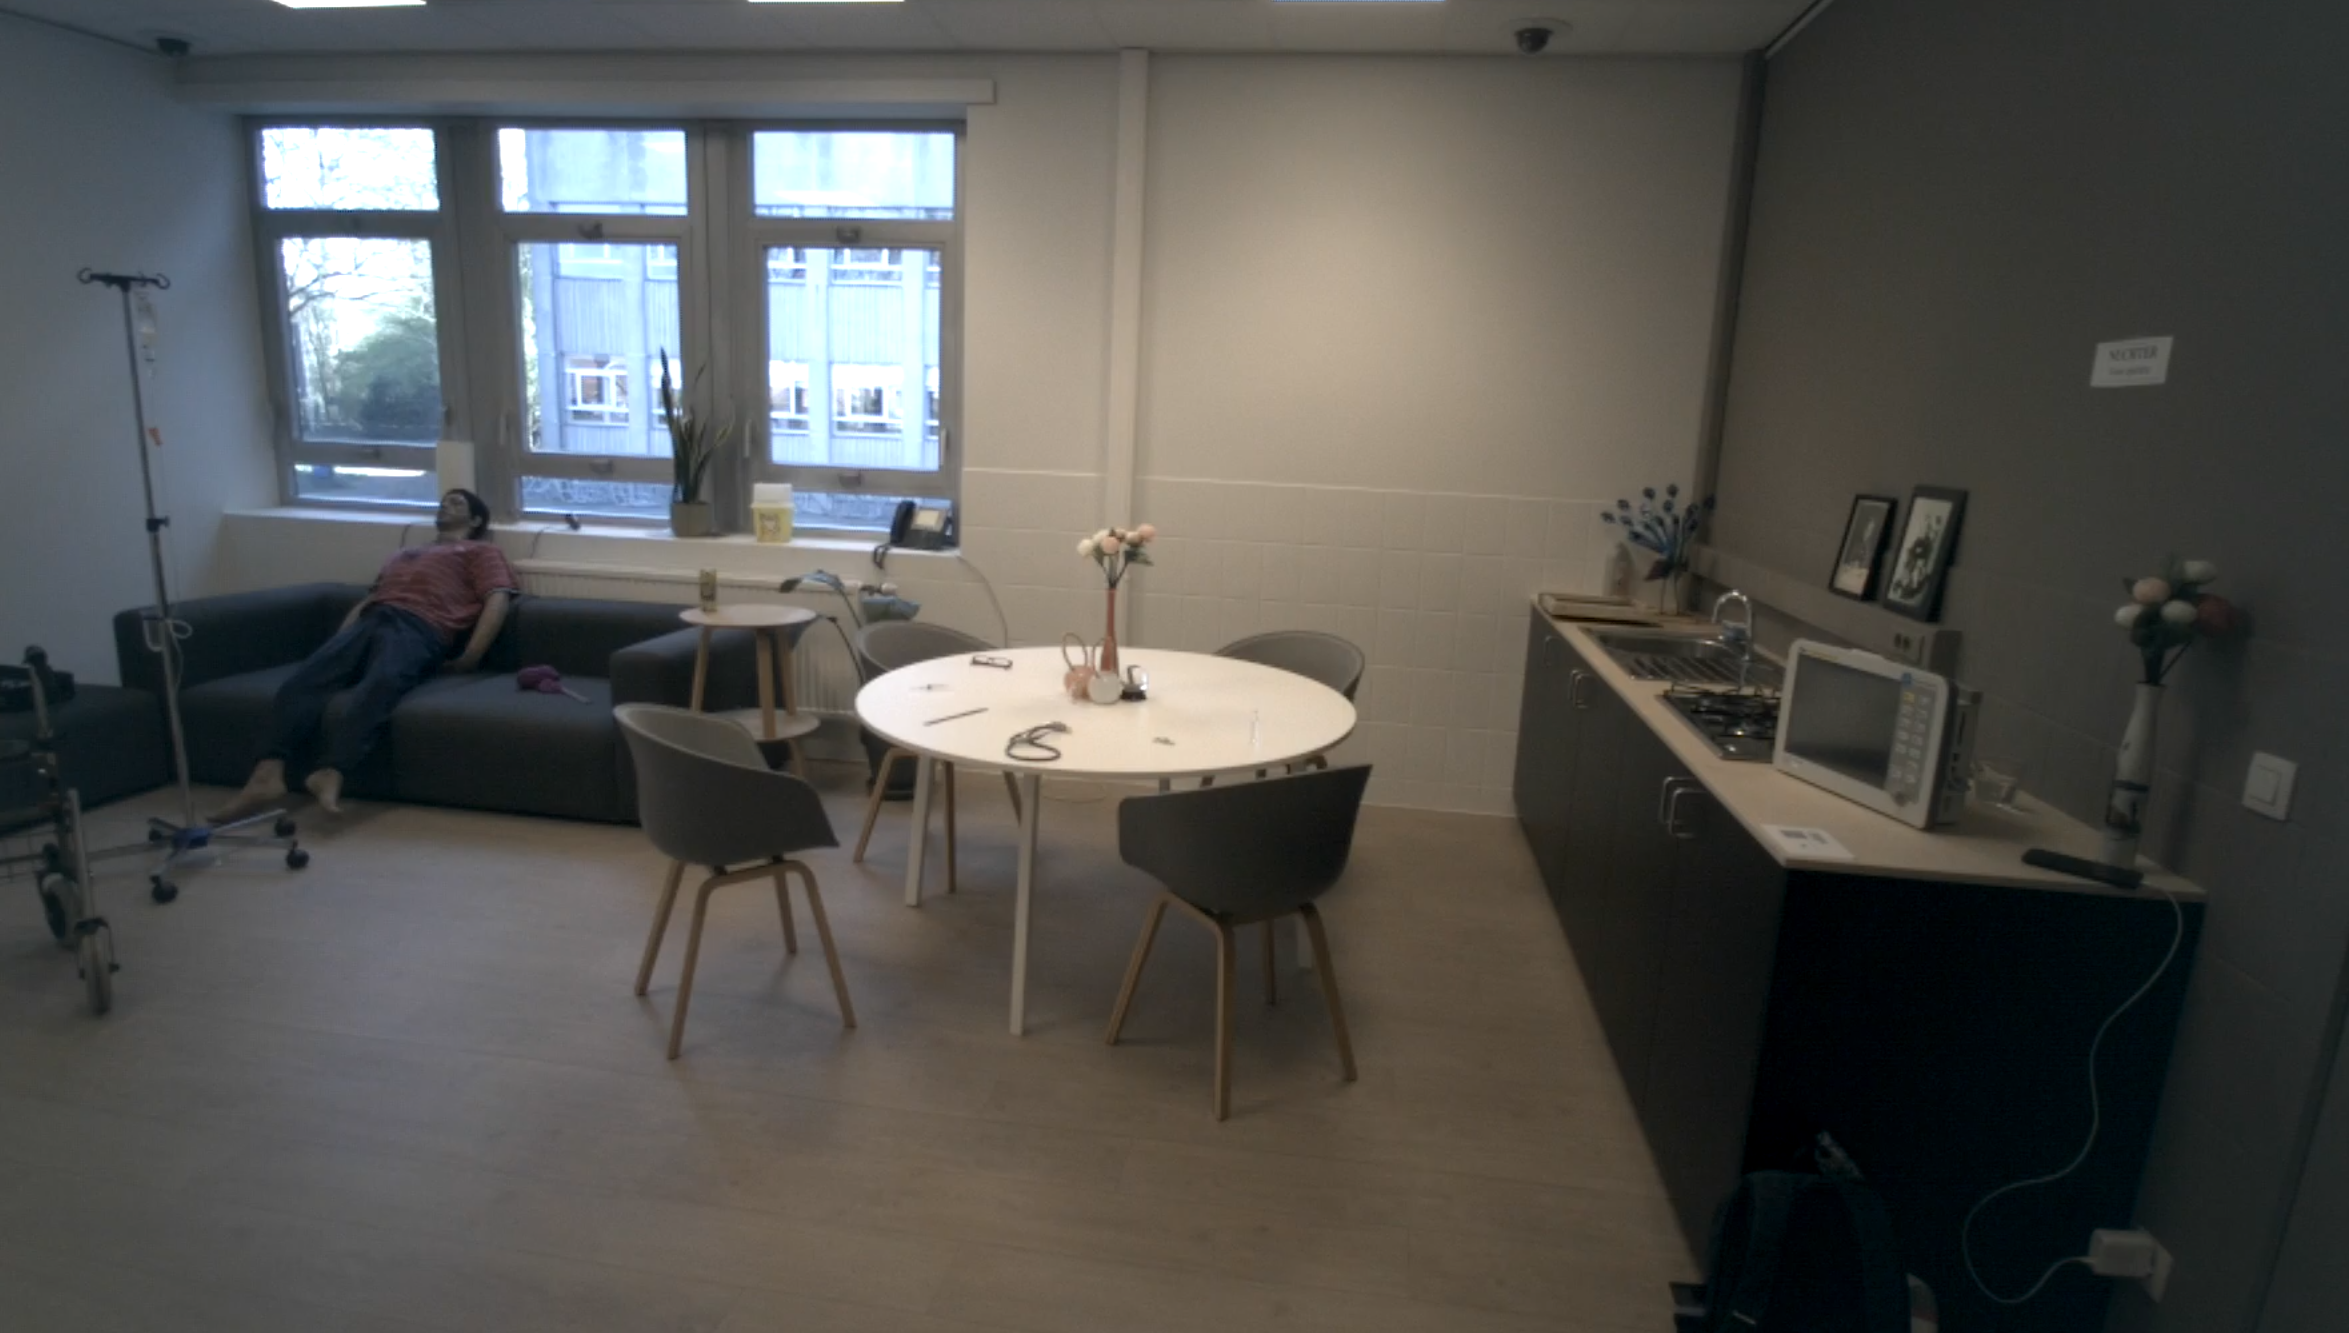
\includegraphics[width=1\textwidth]{zorglab.png}
  \caption[]{\label{fig:zorglab} De woonkameromgeving in het Zorglab van HoGent.}
\end{figure}

Het Zorglab beschikt over een uitgebreid assortiment aan objecten die ingezet kunnen worden tijdens simulatietrainingen. 
Uit deze collectie werden voor dit onderzoek 15 specifieke objecten geselecteerd (zie Figuur~\ref{fig:objecten_experiment}). 

\begin{figure}[H]
  \centering
  \includegraphics[width=1\textwidth]{objecten.png}
  \caption[]{\label{fig:objecten_experiment} }
\end{figure}

